% !TEX root =  paper.tex


\section{Evaluation}
\label{section:evaluation}
To evaluate \toolname, we conducted quantitative
studies aiming at answering the following research questions:\\

\begin{enumerate}[label=\textbf{RQ\arabic*},leftmargin=*]
    \item How effective is \toolname in segmenting web pages?
    \item How efficient is the segmentation process in \toolname?
\end{enumerate}

In the following subsections, we discuss the details of the experiments
that we designed to answer each research question,
together with the results.

\subsection{RQ1: Segmentation Effectiveness}
\label{sec:rq-effectiveness}
For the proposed segmentation approach to be useful and reliable,
it is important to comprehensively assess its effectiveness.
The result of segmentation is a set of 
generated web page segments, $\mathbf{\Psi}$.
Accordingly, we assess the segmentation effectiveness by 
measuring the overlap of each generated segment $\psi \in \mathbf{\Psi}$ to the ground truth,
as will be described in this section.

Furthermore, to put all measurements in perspective,
we compare our results against
the VIPS segmentation technique~\cite{cai2003vips},
which is a quite popular state-of-the-art page segmentation tool~\cite{sleiman2013survey, campus2011web}.
We use the popular Java implementation provided in\footnote{\url{https://github.com/tpopela/vips_java}}.
We use all default configurations, parameters, and thresholds in that implementation.
However, we utilized a different rendering engine in order to make the comparison fair.
The original VIPS configuration uses CSSBox\footnote{\url{http://cssbox.sourceforge.net/}}
as its rendering component, instead of a more common rendering engine such as that of Google Chrome or Mozilla Firefox.
CSSBox's role is equivalent to the web page rendering engine in a web browser.
However, we noted that, out of the box, 
VIPS segmentation was poor due to CSSBox's
inability to properly render modern web pages,
since CSSBox has not been maintained fast enough to keep up with the rapid pace of web technologies,
while the larger scale engines in Google Chrome or Mozilla Firefox are more up to speed.
So we thought that, in order to make the comparison fair for VIPS 
and focused on the actual algorithm rather
than the choice of rendering engine,
we configured VIPS to use the Google Chrome web browser
(via Selenium automation\footnote{\url{https://www.seleniumhq.org/}}).
Google Chrome has, of course, a better industry-quality
rendering engine compared to CSSBox, and therefore our configuration
of VIPS to use Google Chrome instead of CSSBox
is only an improvement of VIPS' quality.
Our proposed tool, \toolname, is also configured to use Google Chrome,
thereby ensuring that any differences in segmentation effectiveness
between the two tools are due to the algorithm itself,
instead of being due to any differences in rendering.


Accordingly, we obtain two sets of web page segments:
~$\mathbf{\Psi^V}$, the set of segments generated by VIPS
and $\mathbf{\Psi^C}$, the set of segments generated by \toolname.
Then, for each segment $\psi^v \in \mathbf{\Psi^V}$ and $\psi^c \in \mathbf{\Psi^C}$,
we compute the \emph{precision}, \emph{recall},
and \emph{F-measure} with respect to ground truth data,
which we now describe.

\header{Ground Truth}
In order to compute the precision and recall, we must first obtain
ground truth data against which the evaluation will be conducted.
Since the output of the proposed segmentation approach is a set of 
web page segments, the ground truth should also contain data 
delineating web page segments.

A basic approach would be to construct ground truth data ourselves
where we manually segment a set of subjects.
However, this approach is biased
and constitutes a threat to the validity of evaluation.
Therefore, we opted for an alternative approach. 
We use a publicly available third party dataset\footnote{\url{https://github.com/rkrzr/dataset-popular}}
that contains random web pages obtained from the Yahoo web directory,
with each page manually analyzed by a group of volunteers and divided into segments. 
A number of subjects had changed locations (i.e., their URLs were dead)
and therefore did not load in the browser and had to be excluded.
There were also other pages for which 
VIPS crashed with null pointer exceptions,
and therefore had to be excluded as well to keep the comparison fair to VIPS.
The final list of ground truth subjects
is shown in \Cref{tbl:evaluation-subjects}.
The table shows the number of DOM nodes and CSS size (in kilobytes)
for the subjects, which gives a rough idea of the complexity of the page.
The table also shows the number of ground truth segments identified in each subject.

\begin{table}
	\caption{Evaluation subjects' descriptive statistics}
	\centering
	%\fontsize{8pt}{9.2pt}\selectfont
	%\setlength\tabcolsep{2px}
	\begin{threeparttable}
		\bgroup
		%\def\arraystretch{1.2}
		\begin{tabular}{r r r r}
			\toprule
			\textbf{Subject\#} & \textbf{\#DOM nodes}	& \textbf{CSS size (KB)}  &  \textbf{\#segments} \\
			\toprule
1 	 & 	 164 	 & 	 87.0 	 & 	 5 	 \\
2 	 & 	 199 	 & 	 42.0 	 & 	 8 	 \\
3 	 & 	 280 	 & 	 23.8 	 & 	 7 	 \\
4 	 & 	 284 	 & 	 181.9 	 & 	 11 	 \\
5 	 & 	 346 	 & 	 13.1 	 & 	 13 	 \\
6 	 & 	 356 	 & 	 23.0 	 & 	 10 	 \\
7 	 & 	 368 	 & 	 86.2 	 & 	 11 	 \\
8 	 & 	 456 	 & 	 55.7 	 & 	 10 	 \\
9 	 & 	 469 	 & 	 303.1 	 & 	 18 	 \\
10 	 & 	 490 	 & 	 10.8 	 & 	 20 	 \\
11 	 & 	 500 	 & 	 63.5 	 & 	 9 	 \\
12	 & 	 524 	 & 	 81.9 	 & 	 9 	 \\
13 	 & 	 557 	 & 	 18.5 	 & 	 13 	 \\
14 	 & 	 611 	 & 	 40.8 	 & 	 8 	 \\
15 	 & 	 629 	 & 	 235.8 	 & 	 19 	 \\
16 	 & 	 636 	 & 	 120.4 	 & 	 16 	 \\
17 	 & 	 665 	 & 	 89.5 	 & 	 6 	 \\
18 	 & 	 714 	 & 	 111.0 	 & 	 22 	 \\
19 	 & 	 748 	 & 	 120.3 	 & 	 18 	 \\
20 	 & 	 772 	 & 	 251.5 	 & 	 12 	 \\
21 	 & 	 893 	 & 	 166.9 	 & 	 8 	 \\
22 	 & 	 908 	 & 	 57.4 	 & 	 21 	 \\
23 	 & 	 932 	 & 	 71.1 	 & 	 21 	 \\
24 	 & 	 942 	 & 	 406.4 	 & 	 16 	 \\
25 	 & 	 955 	 & 	 832.3 	 & 	 14 	 \\
26 	 & 	 1,004 	 & 	 150.9 	 & 	 15 	 \\
27 	 & 	 1,034 	 & 	 280.1 	 & 	 18 	 \\
28 	 & 	 1,068 	 & 	 179.8 	 & 	 6 	 \\
29 	 & 	 1,086 	 & 	 197.7 	 & 	 21 	 \\
30 	 & 	 1,191 	 & 	 117.5 	 & 	 15 	 \\
31 	 & 	 1,398 	 & 	 109.0 	 & 	 16 	 \\
32 	 & 	 1,667 	 & 	 12.9 	 & 	 11 	 \\
33 	 & 	 1,862 	 & 	 96.2 	 & 	 18 	 \\
34 	 & 	 2,344 	 & 	 53.5 	 & 	 12 	 \\
35 	 & 	 2,678 	 & 	 189.7 	 & 	 5 	 \\


\bottomrule

\end{tabular}
\egroup
\end{threeparttable}
\label{tbl:evaluation-subjects}
\end{table}



\header{Measurement}
The measurement of precision and recall is performed as follows.
First, for each test subject,
we obtain the set of segments $\mathbf{\Psi^C}$ generated by \toolname
as well as the set of segments $\mathbf{\Psi^V}$ from VIPS.
We also obtain the set of ground truth segments, $\gamma \in \mathbf{\Gamma}$.
Then, in order to measure the precision and recall, we need to define 
notions of true positive, false positive, and false negative outcomes.

Our definitions are based on treating each generated segment as being composed of two regions:
a true positive region, where the generated segment overlaps with the ground truth segment,
and a false positive region, where the generated segment does not overlap with the ground truth. 
More specifically:

\begin{equation}
    \label{eqn:tp}
    TP = \sum_{\psi \in \mathbf{\Psi}} \vert \psi \cap \eta(\psi) \vert
\end{equation}
where $TP$ is the true positive area and $\eta(\psi) \in \mathbf{\Gamma}$ is the nearest neighbor of 
output segment $\psi$, but from the ground truth set $\mathbf{\Gamma}$. 
We use a nearest neighbor search in order to identify the pairs
of segments that should be compared. 
That is, for each generated segment, which ground truth segment
should be used for measuring precision and recall.
Then, after this pairing, \cref{eqn:tp} sums the areas of intersection
for all pairs. This total area becomes the true positive measure. 

As for false positives, we use the following measure:
\begin{equation}
    \label{eqn:fp}
    FP = \sum_{\psi \in \mathbf{\Psi}} \vert \psi - \eta(\psi) \vert
\end{equation}
in this case, we also begin by finding the nearest neighbor similar
to our true positive calculation in \cref{eqn:tp}.
However, instead of taking the area of intersection between each pair,
we exclude overlapping areas between the pairs, and measure the remaining area.
This measures how much of the generated segment is \emph{not} overlapping
with ground truth, thereby indicating a false positive.
We note that, in case there is no overlap at all between
the generated segment and the ground truth,
then \cref{eqn:fp} correctly measures the \emph{entire} area
of the generated segment as false positive.

The false negative computation differs slightly from the two previous measures
for true and false positives. Because a false negative is, by definition,
absent from the generated segments,
the measurement can not iterate over the output set $\mathbf{\Psi}$ as in
the previous two equations.
Instead, the iteration is performed over the ground truth set $\mathbf{\Gamma}$,
as follows: 
\begin{equation}
    \label{eqn:fn}
    FN = \sum_{\gamma \in \mathbf{\Gamma}} \vert \gamma - \mu(\gamma) \vert
\end{equation}
where $\mu(\gamma) \in \mathbf{\Psi}$ is the nearest neighbor of 
ground truth segment $\gamma$ in the set of output segments $\mathbf{\Psi}$.
This nearest neighbor function $\mu(\gamma)$ acts in an opposite manner to the
preceding nearest neighbor function $\eta(\psi)$ used in equations \ref{eqn:tp} and \ref{eqn:fp}.
$\mu(\gamma)$ pairs a ground truth segment $\gamma$ with the matching output segment $\psi$,
while $\eta(\psi)$ pairs an output segment to a ground truth segment. 
The false negative is then measured as the non-overlapping region of a ground truth segment.
We note that, in case there is no overlap at all between
the ground truth segment and the generated segment,
then the entire area of the ground truth segment is measured as false negative.

To summarize the approach we use to calculate the different measurements,
\Cref{fig:possible-intersections} shows all possible arrangements
of output segments and ground truth segments, and how the true positive, false positive,
and false negative values are defined in each case.

\begin{figure}
    \centering
    {%
    \setlength{\fboxsep}{0pt}%
    \setlength{\fboxrule}{1pt}%
    \fbox{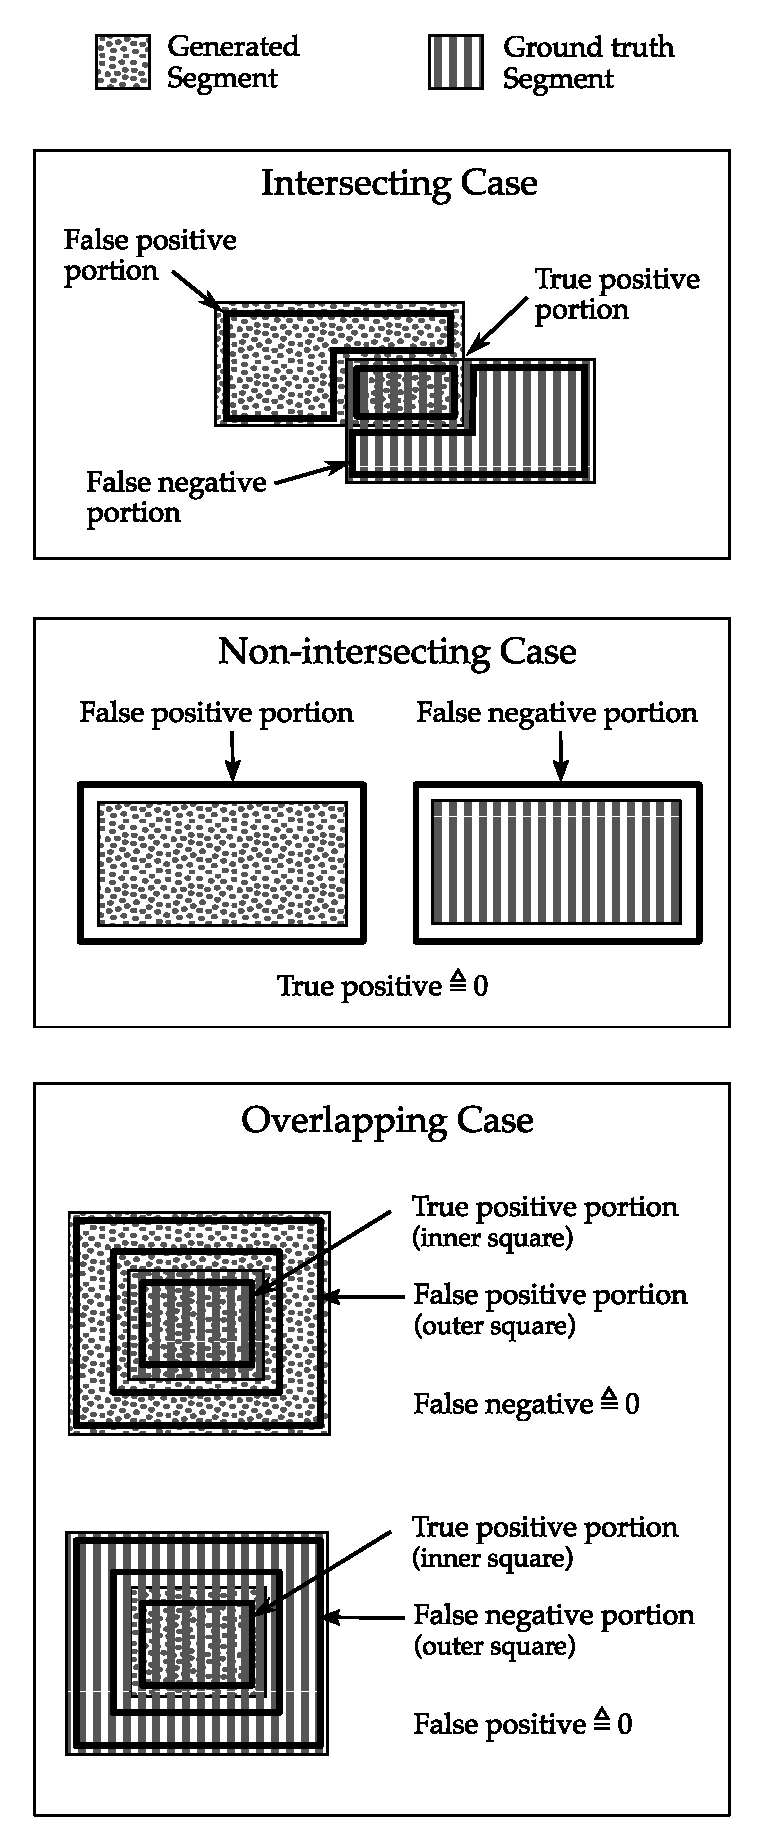
\includegraphics[trim=0 0 0 0,clip,scale=0.55]{figures/evaluation/possible-intersections-fig.pdf}}
    }%
    \caption{Arrangement variations of
    ground truth segments and output segments
    for evaluating segmentation effectiveness.
    %fixed \mohammad{The dotted patterns appear weird dependeing on the pdf viewer. I will change the pattern later.}
    }
    \label{fig:possible-intersections}
\end{figure}


We make one final remark regarding these measurements.
The measurements are performed for the subject \emph{as a whole}.
That is, even though the equations iterate over each segment,
the measure is indicative of the effectiveness
of segmentation for the subject as a whole.
No averaging of any kind is performed
and therefore the final computed precision and recall
represent \emph{exact} as opposed to averaged measurements.

\subsection{RQ2: Efficiency of Segmentation}
We evaluate the efficiency of the segmentation process in order to assess
how computationally expensive is the segmentation.
While segmentation precision and recall is of prime importance,
having a highly accurate segmentation
that is computationally prohibitive makes it practically unusable for real-life web applications.
We therefore believe it is useful to complement the precision evaluation with
an examination of efficiency.

Similar to \Cref{sec:rq-effectiveness},
we also compare the efficiency of \toolname against
that of VIPS and use the same subjects.
In order to ensure a fair comparison, we make a number of remarks.
First, both VIPS and \toolname
were implemented in the same programming language (Java)
to reduce potential efficiency disparities due to programming language choice.
Second, VIPS was configured 
to use Google Chrome (via the Selenium framework),
instead of CSSBox used in the original configuration.
One reason for this choice,
in addition to rendering accuracy issues as mentioned in \Cref{sec:rq-effectiveness},
is to ensure that both tools, VIPS and \toolname,
are using the same browser engine in order to neutralize any potential
differences in efficiencies pertaining to web page rendering or DOM access.

\header{Measurement}
We measure the execution time as follows.
First, we launch browser sessions and load a test subject.
None of these steps are timed as they are outside the scope of segmentation 
and are also necessary prerequisites to any segmentation tool.
Next, we prepare and/or cast the variables in the expected classes and formats
required by each tool. None of these steps are timed either, since they
occur before the segmentation execution itself.
After all required inputs are ready, we run the segmentation and begin the timing process.
Once all segments are generated and available for use, we stop timing.





